\documentclass[11pt,letterpaper]{article}
\usepackage[utf8]{inputenc}
\usepackage{amsmath}
\usepackage{amsfonts}
\usepackage{amssymb}
\usepackage{geometry}
\usepackage{hyperref}
\usepackage{xcolor}
\usepackage{booktabs}
\usepackage{multicol}
\usepackage{caption}
\usepackage{float}
\usepackage{graphicx}
\graphicspath{{visual-assets/}}

% Brand Typography / Color configuration
\definecolor{mpdark}{HTML}{0F172A}
\definecolor{mpblue}{HTML}{3B82F6}
\definecolor{mpgreen}{HTML}{10B981}
\definecolor{mpred}{HTML}{EF4444}
\definecolor{mppurple}{HTML}{8B5CF6}
\definecolor{mpamber}{HTML}{F59E0B}
\definecolor{mpgrey}{HTML}{64748B}

\geometry{margin=1in}

\hypersetup{
    colorlinks=true,
    linkcolor=mpblue,
    urlcolor=mpblue
}

\setlength{\abovedisplayskip}{4pt}
\setlength{\belowdisplayskip}{4pt}
\setlength{\abovedisplayshortskip}{2pt}
\setlength{\belowdisplayshortskip}{2pt}

\title{\vspace{-20pt}\textbf{\color{mpdark}Money Plot Labs Technical Whitepaper 003 \\
From Determinism to Probability: \\
The Stochastic Retirement Framework}}
\author{\textbf{Harrison Hsueh} \\ \textit{Founder, Money Plot Labs}}
\date{May 2026}

\begin{document}

\maketitle

\begin{abstract}
\vspace{-5pt}
Whitepapers 001 and 002 derived exact closed-form solutions for retirement timelines under \emph{deterministic} real growth rates. This paper lifts that constraint and introduces a fully stochastic framework. We establish the lognormal portfolio model, derive the It\^{o} correction linking arithmetic mean to median compound growth, and show how the standard normal quantile function yields closed-form percentile retirement dates without simulation. For portfolios with cash flows, we introduce the Fenton-Wilkinson lognormal moment-matching approximation. Together these tools allow the \emph{p10 retirement age} --- the year a saver can retire while remaining solvent in 90\% of all historical market environments --- to be computed analytically in milliseconds.
\end{abstract}

% =========================================================================
\section{Motivation: Why Determinism is Insufficient}
% =========================================================================

Whitepaper 001 derived a beautiful closed-form expression for the required working years~$w$:
\begin{equation}
w = H - \frac{\ln \!\left[\dfrac{(rA_0 + s)(1+r)^H + c(1+r) - rL}{s + c(1+r)}\right]}{\ln(1+r)}
\end{equation}

This formula is exact --- given a fixed real growth rate~$r$. The problem is that real investment returns are not fixed. A 60/40 portfolio has delivered a long-run arithmetic mean of $\mu = 5.9\%$, but with a standard deviation of $\sigma = 12.5\%$. A saver who plugs $r = 5.9\%$ into Equation~(1) will compute a retirement date that is achievable in roughly 50\% of historical environments --- and catastrophically optimistic in the other 50\%.

The stochastic framework presented here answers a more honest question: \emph{How many years must I work so that I can retire in 90\% of all possible market environments?} This is the p10 retirement age, and it has a clean analytical derivation.

% =========================================================================
\section{The Lognormal Portfolio Model}
% =========================================================================

\subsection{The Basic Setup}

Let $r_t$ denote the real annual return in year~$t$, drawn independently from a distribution with arithmetic mean~$\mu$ and standard deviation~$\sigma$. For a portfolio with no cash flows and initial value~$A_0$, the value after $n$ years is:
\begin{equation}
A_n = A_0 \prod_{t=1}^{n} (1 + r_t)
\end{equation}

Taking logarithms:
\begin{equation}
\ln A_n = \ln A_0 + \sum_{t=1}^{n} \ln(1 + r_t)
\end{equation}

Each log-return $\ln(1+r_t)$ is approximately normally distributed. By the Central Limit Theorem, the sum of $n$ i.i.d. terms converges to:
\begin{equation}
\ln A_n \;\sim\; \mathcal{N}\!\left(\ln A_0 + n\mu_\ell,\;\; n\sigma_\ell^2\right)
\end{equation}

where the \textbf{log-return parameters} are:
\begin{equation}
\mu_\ell \;=\; \ln(1+\mu) - \frac{\sigma^2}{2(1+\mu)^2} \;\approx\; \mu - \frac{\sigma^2}{2}
\label{eq:mu_l}
\end{equation}
\begin{equation}
\sigma_\ell^2 \;=\; \ln\!\left(1 + \frac{\sigma^2}{(1+\mu)^2}\right) \;\approx\; \frac{\sigma^2}{(1+\mu)^2}
\label{eq:sigma_l}
\end{equation}

Equation~(\ref{eq:mu_l}) is the celebrated \textbf{It\^{o} correction}. The log-mean $\mu_\ell$ is strictly less than $\mu$: higher volatility \emph{always} reduces the median compound growth rate below the arithmetic mean. This is not a modeling choice --- it is a mathematical identity.

\subsection{The It\^{o} Correction in Practice}

For the 60/40 portfolio ($\mu = 5.9\%$, $\sigma = 12.5\%$):
\begin{equation}
\mu_\ell \;\approx\; 5.9\% - \frac{(0.125)^2}{2} \;=\; 5.9\% - 0.78\% \;=\; \mathbf{5.12\%}
\end{equation}

The median CAGR is $e^{\mu_\ell} - 1 \approx 5.25\%$ --- not 5.9\%. A saver who plans on the arithmetic mean will find themselves in the bottom half of all outcomes.

\begin{figure}[H]
\centering
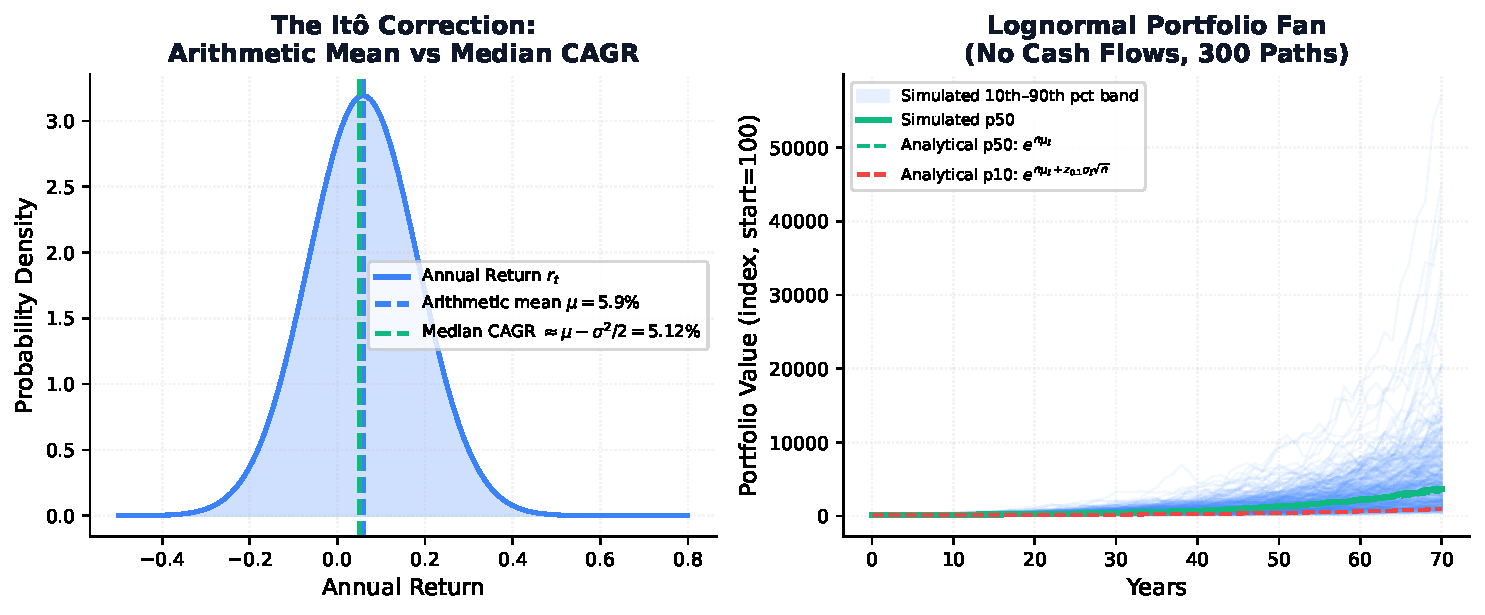
\includegraphics[width=13cm]{lognormal_fan.pdf}
\caption{\textbf{Left:} The It\^{o} gap between arithmetic mean $\mu$ (dashed \textcolor{mpblue}{blue}) and median CAGR $\mu - \sigma^2/2$ (dashed \textcolor{mpgreen}{green}). \textbf{Right:} 300 simulated portfolio paths (no cash flows) with analytical percentile bounds overlaid. The p50 and p10 analytical curves match the simulation fan precisely, confirming the lognormal model.}
\end{figure}

% =========================================================================
\section{Closed-Form Percentile Portfolio Value}
% =========================================================================

Since $\ln A_n \sim \mathcal{N}(\ln A_0 + n\mu_\ell,\; n\sigma_\ell^2)$, the $p$-th percentile portfolio value at year $n$ is:
\begin{equation}
\boxed{A_n^{(p)} = A_0 \cdot \exp\!\left(n\mu_\ell + \sqrt{n}\,\sigma_\ell \cdot z_p\right)}
\label{eq:pct_path}
\end{equation}

where $z_p = \Phi^{-1}(p/100)$ is the standard normal quantile ($z_{0.10} = -1.282$, $z_{0.50} = 0$, $z_{0.90} = +1.282$). This is an exact closed-form expression --- no simulation required.

The p10 portfolio ($z_{0.10} = -1.282$) after $n$ years is therefore:
\begin{equation}
A_n^{(10)} = A_0 \cdot \exp\!\left(n\mu_\ell - 1.282\sqrt{n}\,\sigma_\ell\right)
\end{equation}

% =========================================================================
\section{The Closed-Form Percentile Retirement Date}
% =========================================================================

\subsection{No Cash Flows Case}

Set $A_n^{(p)} = F$ (the target nest egg) and solve for~$n = w$. From Equation~(\ref{eq:pct_path}):
\begin{equation}
\ln(F/A_0) = w\mu_\ell + z_p\,\sigma_\ell\,\sqrt{w}
\end{equation}

This is a quadratic equation in $u = \sqrt{w}$:
\begin{equation}
\mu_\ell\, u^2 + z_p\,\sigma_\ell\, u - \ln(F/A_0) = 0
\end{equation}

Applying the quadratic formula (taking the positive root):
\begin{equation}
\boxed{u = \frac{-z_p\sigma_\ell + \sqrt{z_p^2\sigma_\ell^2 + 4\mu_\ell\ln(F/A_0)}}{2\mu_\ell}, \qquad w = u^2}
\label{eq:quadratic}
\end{equation}

\noindent This is a \textbf{complete closed-form solution} for the $p$-th percentile retirement date under lognormal returns with no cash flows. To compute the p10 retirement date, substitute $z_p = -1.282$.

\subsection{The Effective Discount Rate Interpretation}

Equation~(\ref{eq:quadratic}) can be recast as: the p-th percentile retirement date is \emph{equivalent} to running the deterministic Whitepaper 001 formula with an effective real growth rate:
\begin{equation}
\boxed{r_{\text{eff}}^{(p)}(w) = \exp\!\left(\mu_\ell + \frac{z_p\,\sigma_\ell}{\sqrt{w}}\right) - 1}
\label{eq:reff}
\end{equation}

This expression reveals a critical structural insight: the effective rate that produces the $p$-th percentile outcome is \textbf{horizon-dependent}. For short horizons (small~$w$), the volatility penalty $z_p\sigma_\ell/\sqrt{w}$ is large and the p10 effective rate is severely depressed. As the horizon grows, the penalty shrinks as $1/\sqrt{w}$ and the effective rate converges toward $\mu_\ell$. This is the mathematical signature of time-diversification of volatility.

\noindent\textbf{Example (60/40 portfolio, $w = 30$ years):}
\begin{align*}
r_{\text{eff}}^{(10)}(30) &= \exp\!\left(0.0512 + \frac{(-1.282)(0.118)}{\sqrt{30}}\right) - 1 \\
                          &= \exp\!\left(0.0512 - 0.0276\right) - 1 \\
                          &\approx \mathbf{2.39\%}
\end{align*}

A planner targeting p10 safety over a 30-year horizon should use an effective rate of 2.39\% --- not the arithmetic mean of 5.9\%, and not even the median CAGR of 5.25\%.

% =========================================================================
\section{The Fenton-Wilkinson Approximation with Cash Flows}
% =========================================================================

\subsection{Why Cash Flows Break the Closed Form}

With annual savings~$s$, the portfolio value is:
\begin{equation}
A_n = A_0\prod_{t=1}^n R_t + s\sum_{k=1}^n \prod_{t=k+1}^n R_t, \qquad R_t = 1 + r_t
\end{equation}

This is a sum of lognormal random variables. A sum of lognormals is \emph{not} lognormal in general, so Equation~(\ref{eq:pct_path}) no longer applies exactly. The Fenton-Wilkinson (FW) method fits a lognormal to the distribution of~$A_n$ by matching its first two moments analytically.

\subsection{Moment Recursion}

Define $\mathbb{E}[A_n]$ and $\mathbb{E}[A_n^2]$ via the following one-step recursion. Starting from $A_0$:
\begin{align}
\mathbb{E}[A_{t+1}] &= \mathbb{E}[A_t]\,(1 + \mu) + s \label{eq:mean_rec}\\
\mathbb{E}[A_{t+1}^2] &= \mathbb{E}[A_t^2]\,(1+\mu)^2 e^{\sigma_\ell^2} + 2\,\mathbb{E}[A_t]\,s\,(1+\mu) + s^2 \label{eq:var_rec}
\end{align}

From these, $\text{Var}[A_n] = \mathbb{E}[A_n^2] - (\mathbb{E}[A_n])^2$.

\subsection{Fitting the Lognormal (FW Parameters)}

Given $\mathbb{E}[A_n]$ and $\text{Var}[A_n]$, fit $\ln A_n \sim \mathcal{N}(m_n, v_n^2)$ by matching moments:
\begin{equation}
m_n = 2\ln\mathbb{E}[A_n] - \tfrac{1}{2}\ln\!\left(\text{Var}[A_n] + \mathbb{E}[A_n]^2\right)
\end{equation}
\begin{equation}
v_n = \sqrt{\ln\!\left(1 + \dfrac{\text{Var}[A_n]}{\mathbb{E}[A_n]^2}\right)}
\end{equation}

The $p$-th percentile portfolio value at year~$n$ with cash flows is then:
\begin{equation}
\boxed{A_n^{(p)} \;\approx\; \exp\!\left(m_n + z_p\, v_n\right)}
\label{eq:fw_pct}
\end{equation}

\begin{figure}[H]
\centering
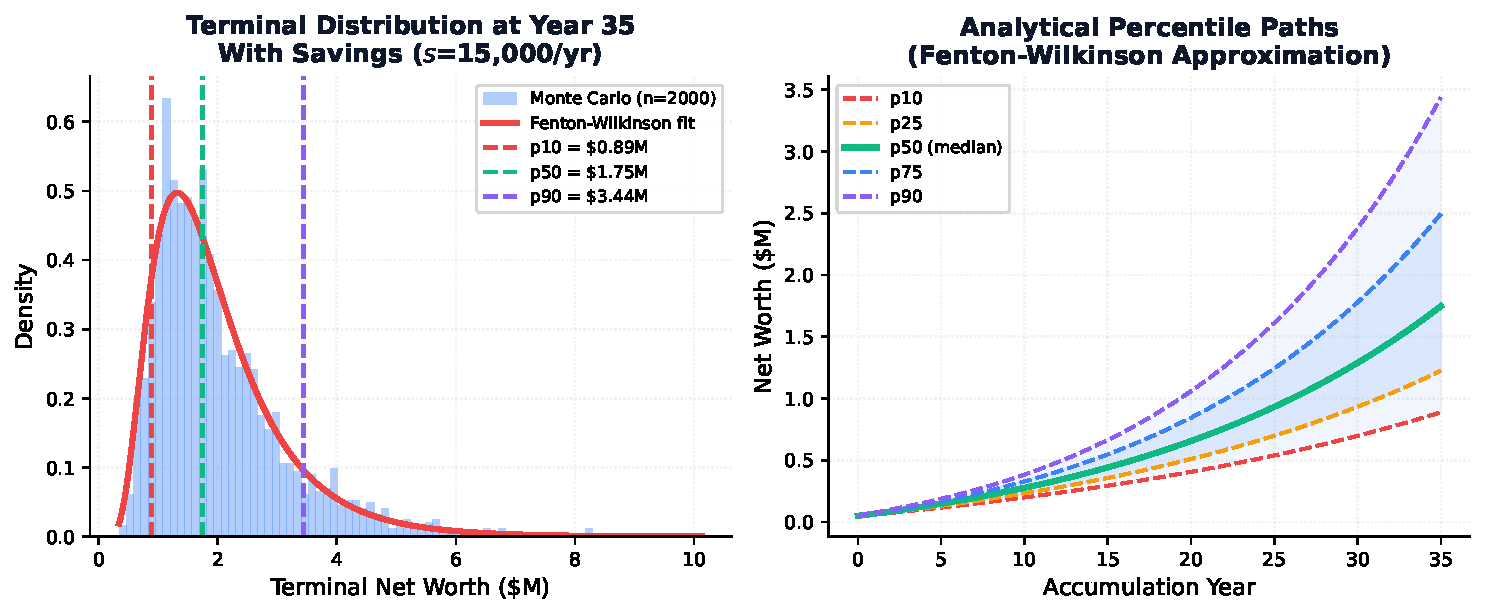
\includegraphics[width=13cm]{fenton_wilkinson.pdf}
\caption{\textbf{Left:} Terminal distribution after 35 accumulation years with $s=\$15{,}000$/yr. The Fenton-Wilkinson fitted lognormal ({\color{mpred}red}) closely tracks the Monte Carlo histogram ({\color{mpblue}blue}). \textbf{Right:} Analytical percentile NW paths over the accumulation phase. The fan widens non-linearly: variance grows as $\sqrt{n}$ in log-space, compressing early and spreading late.}
\end{figure}

\subsection{Percentile Retirement Date with Cash Flows}

To find the p-th percentile working years $w$ when saving $s$ per year, invert Equation~(\ref{eq:fw_pct}): find the smallest $w$ such that $A_w^{(p)} \geq F$. Since the FW parameters $m_n, v_n$ are computed via the recursion~(\ref{eq:mean_rec})--(\ref{eq:var_rec}), this requires a simple binary search over~$w$ --- but each evaluation is $O(w)$ arithmetic operations and involves no random sampling. For a 70-year horizon this is instantaneous.

% =========================================================================
\section{Unified Summary Table}
% =========================================================================

\begin{table}[H]
\centering
\small
\begin{tabular}{llll}
\toprule
\textbf{Setting} & \textbf{Cash Flows} & \textbf{Method} & \textbf{Retirement Date} \\
\midrule
Constant $r$ & Any & Whitepaper 001 Eq.\,(28) & Exact closed form \\
Stochastic, no CF & $s=0$ & Quadratic Eq.\,(\ref{eq:quadratic}) & Exact closed form \\
Stochastic, with CF & Any $s$ & FW recursion + binary search & Near-instantaneous \\
Empirical returns & Any & Monte Carlo (bootstrap/cohort) & Stress Tester tool \\
\bottomrule
\end{tabular}
\caption{Four levels of the retirement timeline problem, from algebraic to stochastic.}
\end{table}

% =========================================================================
\section{The Convergence to Determinism}
% =========================================================================

A key sanity check: as $\sigma \to 0$, $\sigma_\ell \to 0$, and the percentile retirement date becomes horizon-independent and collapses to a single value regardless of~$p$. The effective rate Equation~(\ref{eq:reff}) collapses to $r_{\text{eff}} = e^{\mu_\ell} - 1 \approx \mu$. The stochastic framework recovers the deterministic Whitepaper 001 result exactly.

A second check: as $n \to \infty$, the volatility penalty $z_p\sigma_\ell/\sqrt{n} \to 0$ and all percentile paths converge to the same median CAGR. This is the time-diversification theorem --- volatility matters less over longer horizons, but it never disappears entirely.

% =========================================================================
\section{Practical Implications for the Stress Tester}
% =========================================================================

The stochastic framework provides two complementary instruments:

\begin{enumerate}
    \item \textbf{The Monte Carlo Stress Tester} (Tool 4) samples directly from 97 years of real historical returns (1928--2024, inflation-adjusted) using either bootstrap resampling or chronological cohort windows. This provides empirically grounded percentile fans that respect the actual fat tails, autocorrelation, and regime structure of historical markets. It does \emph{not} assume lognormality.

    \item \textbf{The Analytical Framework} (this paper) assumes i.i.d.\ lognormal returns and derives percentile retirement dates in closed form. It is exact for the no-cash-flow case and highly accurate via Fenton-Wilkinson for the savings case. It provides instant sensitivity analysis and clear intuition for how volatility, mean, and horizon trade off.
\end{enumerate}

The two instruments are complementary: the analytical framework provides instant intuition, and the Monte Carlo engine provides empirical ground truth. A p10 retirement date that agrees between both methods is robust. A gap between them signals model risk worth examining.

\begin{figure}[H]
\centering
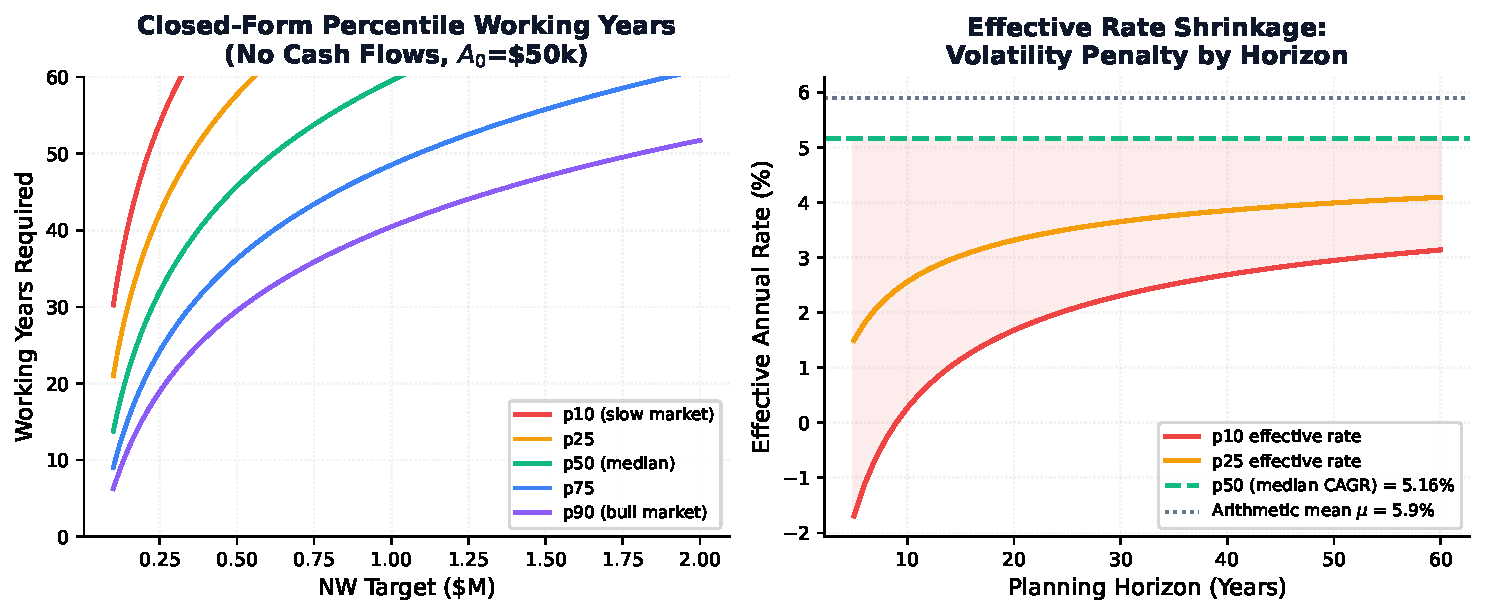
\includegraphics[width=13cm]{percentile_retirement.pdf}
\caption{\textbf{Left:} Closed-form percentile working years vs NW target (no cash flows). The p10 scenario (\textcolor{mpred}{red}) requires substantially more working years than the median (\textcolor{mpgreen}{green}). \textbf{Right:} The effective discount rate by horizon for each percentile. All curves converge to the median CAGR as the horizon grows --- the mathematical expression of time-diversification --- but the penalty is severe at short horizons.}
\end{figure}

% =========================================================================
\section{Data Attribution}
% =========================================================================

All historical return series used in the Stress Tester tool (and as calibration inputs for $\mu$ and $\sigma$ in this paper) cover 1928--2024 (97 years) and are expressed as \textbf{real (inflation-adjusted) annual returns}. Nominal equity and bond returns sourced from \href{https://pages.stern.nyu.edu/~adamodar/New_Home_Page/datafile/histretSP.html}{Aswath Damodaran, NYU Stern}. CPI deflation applied using U.S.\ Bureau of Labor Statistics data.

\begin{table}[H]
\centering
\small
\begin{tabular}{lccc}
\toprule
\textbf{Asset} & \textbf{Arith.\ Mean $\mu$} & \textbf{Std Dev $\sigma$} & \textbf{Geometric CAGR} \\
\midrule
US Equities (S\&P 500) & 8.8\% & 19.6\% & 6.9\% \\
60/40 Portfolio        & 5.9\% & 12.5\% & 5.1\% \\
\bottomrule
\end{tabular}
\caption{Real return statistics used to calibrate the stochastic model, 1928--2024.}
\end{table}

\end{document}
